%-------------------------------------------------------------------------------
%                             ADDITIONAL PACKAGES
%-------------------------------------------------------------------------------
\documentclass[
  letterpaper, 
%   showframes,
%   vline=2.2em,
  maincolor=black,
  sectioncolor=black!90,
  subsectioncolor=black!70,
  itemtextcolor=black!40,
%   sidebarwidth=0.4\paperwidth,
%   topbottommargin=0.03\paperheight,
%   leftrightmargin=20pt,
%   proilepicsize=4.5cm,
]{fortysecondscv}


\usepackage[T1]{fontenc}
\usepackage[utf8]{inputenc}


\usepackage[spanish]{babel}
\usepackage{graphicx}
\usepackage{fancyhdr}
\usepackage{blindtext}
\usepackage{geometry}
\usepackage{array}
\usepackage{multicol}
\usepackage{vwcol} 
\usepackage{tabulary}
\usepackage{url}
\usepackage{float}

% improve word spacing and hyphenation
\usepackage{microtype}
\usepackage{ragged2e}

% take care of proper font encoding
\ifxetexorluatex
	\usepackage{fontspec}
	\defaultfontfeatures{Ligatures=TeX}
% \newfontfamily\headingfont[Path = fonts/]{segoeuib.ttf} % local font
\else
	\usepackage[utf8]{inputenc}
	\usepackage[T1]{fontenc}
% \usepackage[sfdefault]{noto} % use noto google font
\fi

% enable mathematical syntax for some symbols like \varnothing
\usepackage{amssymb}

% bubble diagram configuration
\usepackage{smartdiagram}
\smartdiagramset{
  % defaut font size is \large, so adjust to harmonize with sidebar layout
  bubble center node font = \footnotesize,
  bubble node font = \footnotesize,
  % default: 4cm/2.5cm; make minimum diameter relative to sidebar size
  bubble center node size = 0.4\sidebartextwidth,
  bubble node size = 0.25\sidebartextwidth,
  distance center/other bubbles = 1.5em,
  % set center bubble color
  bubble center node color = maincolor!70,
  % define the list of colors usable in the diagram
  set color list = {maincolor!10, maincolor!40,
  maincolor!20, maincolor!60, maincolor!35},
  % sets the opacity at which the bubbles are shown
  bubble fill opacity = 0.8,
}


%-------------------------------------------------------------------------------
%                            PERSONAL INFORMATION
%-------------------------------------------------------------------------------
%%
%
% \cvprofilepic{img/logoUCR.png}

\cvname{\begin{center}
\includegraphics[width=0.5\textwidth]{img/logoUCR.png}
\\\vspace{-0mm}Universidad de\\Costa Rica\end{center}}

\cvjobtitle{\begin{center}
\includegraphics[width=0.5\textwidth]{img/logoEIE.png}\\\vspace{-0mm}Escuela de\\Ingeniería Eléctrica\end{center}}

%% optional information


% NOTE: ordering in sidebar will mimic the following order
% date of birth
% \cvbirthday{\textit{M. Sc.} Ricardo Román-Brenes}
% short address/location, use \newline if more than 1 line is required
% \cvaddress{\url{ricardo.roman@ucr.ac.cr}}
% phone number


%-------------------------------------------------------------------------------
%                              SIDEBAR 1st PAGE
%-------------------------------------------------------------------------------
% add more profile sections to sidebar on first page
\addtofrontsidebar{
	% include gosquare national flags from https://github.com/gosquared/flags;
	% naming according to ISO 3166-1 alpha-2 country codes

	% social network accounts incl. proper hyperlinks
	\profilesection{Estudiante}
		\begin{icontable}{2em}{1em}
		    % overleaf still not supports Academicons and FontAwesome5 for XeLaTeX, which contain the overleaf logl...unbelievable...
		    %\social{\aiOverleafSquare}
			\social{\faUser}
				{}
				{\textit{} Gabriel Araya Mora}
			\social{\faAt}
				{}
				{\url{gabomora2200@gmail.com}}
		\end{icontable}
		

	 
       
    
}

\addtobacksidebar{
	% include gosquare national flags from https://github.com/gosquared/flags;
	% naming according to ISO 3166-1 alpha-2 country codes

	% social network accounts incl. proper hyperlinks
	\profilesection{Docente}
		\begin{icontable}{2.5em}{1em}
		    % overleaf still not supports Academicons and FontAwesome5 for XeLaTeX, which contain the overleaf logl...unbelievable...
		    %\social{\aiOverleafSquare}
			\social{\faUser}
				{}
				{\textit{M. Sc.} Ricardo Román-Brenes}
			\social{\faAt}
				{}
				{\url{ricardo.roman@ucr.ac.cr}}
		\end{icontable}
		
}


%-------------------------------------------------------------------------------
%                         TABLE ENTRIES RIGHT COLUMN
%-------------------------------------------------------------------------------
\begin{document}

\makefrontsidebar


\cvsection{\Huge \texttt{IE-0117} \textbf{Programacion bajo plataformas abiertas}}
\cvsubsection{\huge Laboratorio 1: Linux (Parte1)}
% \begin{cvtable}[1.5]
% 	\cvitem{2009 -- 2010}{Post-Doc Panda Studies}{Panda Academy}
% 		{In-depth studies on the impact of bamboo nutrition for young pandas and
% 		its relation to relaxing, sleeping and snoozing parts of the day.}
% 	\cvitem{2008 -- 2009}{Research Stay Europe}{European Panda Labs}
% 		{Spending one year abroad teaching european panda facilities about the
% 		newest findings and research in the field of asian rice hat covers and
% 		applications for bamboo as a material.}
% \end{cvtable}

% \cvsignature
\section{Instalación}
\subsection{¿Corre en mi sistema?}
    La computadora usada para instalar Linux cuenta con un CPU Intel Core i5 de 7ma generación el cual según la documentación de linux es compatible. \\
    (Intel 386SX/DX/SL, 486SX/DX/SL/SX2/DX2/DX4, Pentium, Pentium Pro, Pentium II, Pentium III (regular and Xeon versions), Pentium 4, and Celeron (including mobile versions of all of the above) are all supported.)
\subsection{¿Qué tipo de teclado tiene?}
    El teclado con el cual cuenta la computadora usada para instalar Linux es de 105 teclas y está configurado en inglés.\\
    Mientras que el mouse con el que se está trabajando no es ni serial ni paralelo ya que está conectado a una entrada USB. 
\subsection{¿Se instalará una estación de trabajo básica o un servidor?}
    Se está usando una máquina virtual (VMWARE) en la cual se instaló el sistema operativo de UBUNTU, el cual trae en su paquete de instalación todas las librerias necesarias para trabajar.
 
\subsection{¿Desde donde instalará Linux?}
    Para esta tarea se booteo previamente un dispositivo USB con el instalador de Linux en ella, para esto es necesario indicarle al BIOS que busque el programa de inicio aquí y no en el disco duro (HDDR). 
\subsection{¿Linux estará solo en la computadora o será necesario crear una partición?}
    En las computadoras de la Universidad se instaló usando una partición, mientras que en la computadora de escritorio de la casa se usó una máquina virtual en lugar de particionar el disco, ya que en los dos casos Windows es el sistema operativo principal en el sistema.
\subsection{¿Está esta computadora conectada a una red?¿Cuál es el nombre y la direccion IP?}
    El equipo se encuentra instalado en una ubicación que cuenta con un punto de acceso inalámbrico a la red doméstica de internet con un ancho de banda de 4Mb/s. El nombre del equipo es Gabriel Araya Mora y la dirección IP es (192.168.50.255). Para hallar la misma se usó le comando ip addr show.
    \begin{figure}[H]
        \centering
        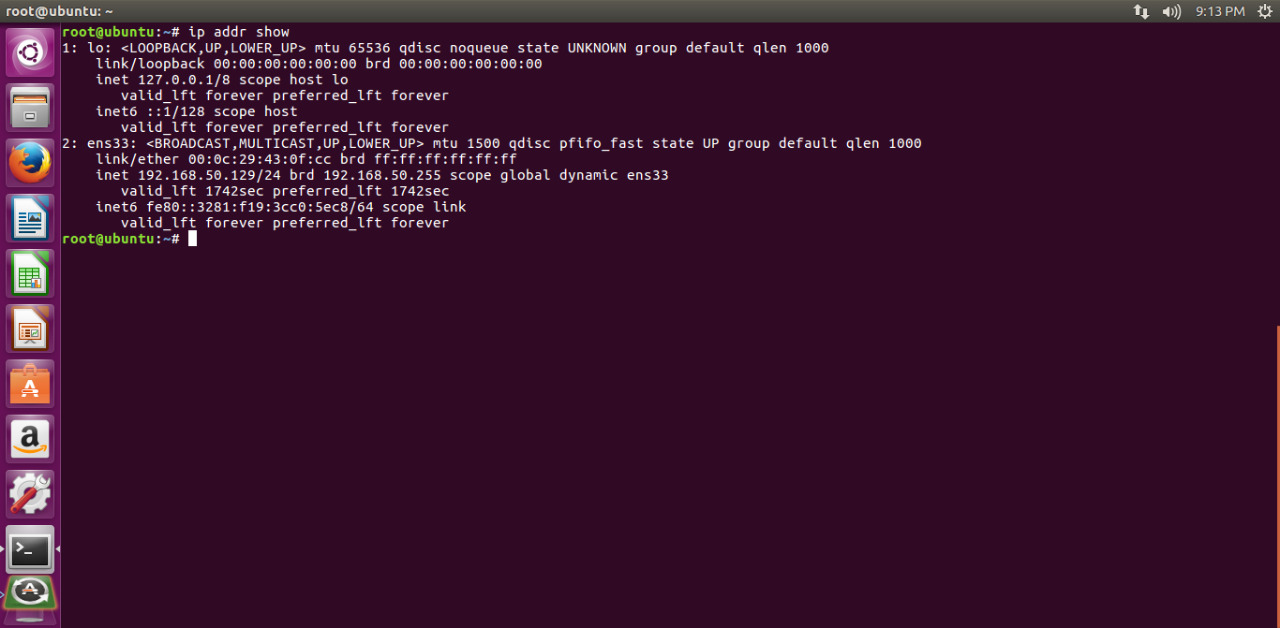
\includegraphics[trim= 0 370 335 0,clip,width=0.95\textwidth]{img/IPLAb.jpg}
        \caption{Hallando Dirección IP}
        \label{fig:my_label}
    \end{figure}
\subsection{¿Es esta computadora un Gateway/Router/Firewall?}
    No, el equipo es un computador de uso personal.
\subsection{Particiones}
    Las particiones en el Laboratorio ya estaban hechas para cuando se instaló el sistema operativo, fue suficiente indicarle al Linux indicarle en cual partición debia alojarse.

\subsection{¿El equipo se inicia en modo Texto o modo Gráfico?}
    Hoy la mayoría de sistemas incian en modo Gráfico, este modo da una salida que genera una imagen usando pixeles, mientras que el modo texto solo permite al usuario escribir. Linux se inicia en modo gráfico pero en consola se trabaja en modo texto.
\subsection{Piense en una clave para el usuario y cree un usuario que no tenga acceso al root}
    La clave del usuario principal llamado Gabriel es: esmeralda, mientras que el usuario con acceso limitado se llamará peon y su clave será su mismo nombre. Para esto de debe usar el comando sudo adduser <nombre>.
    \begin{figure}[H]
        \centering
        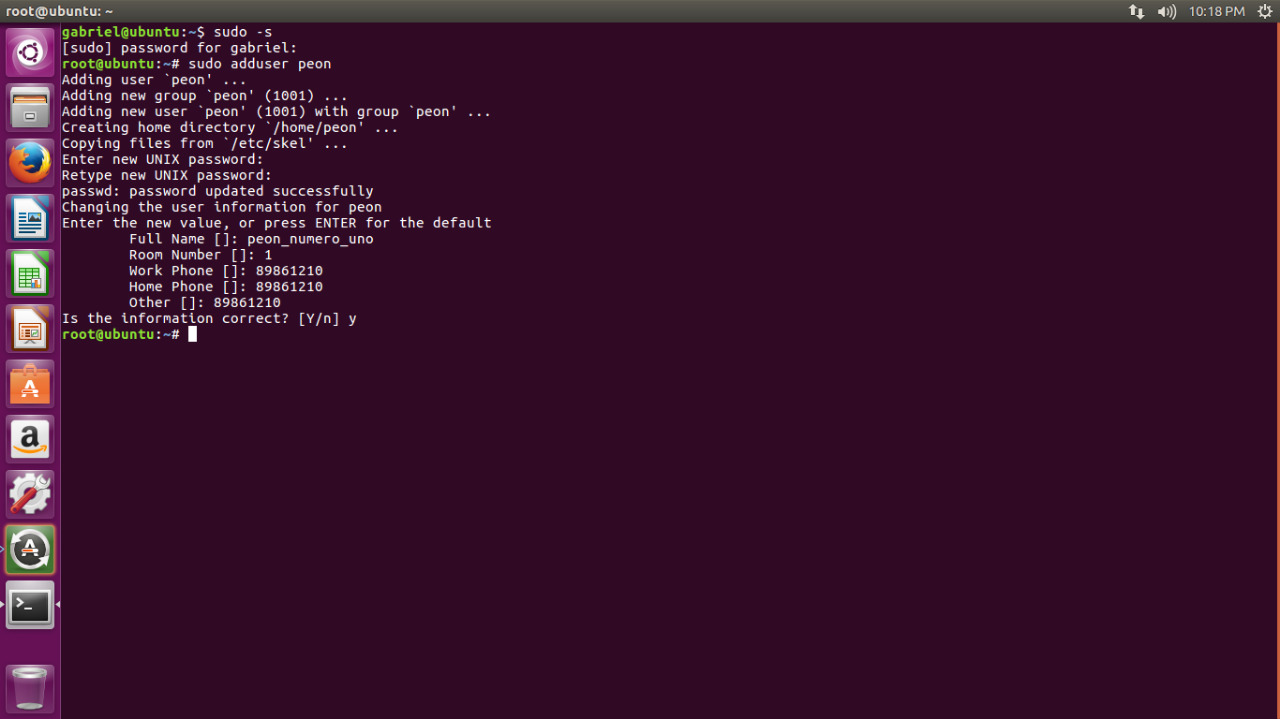
\includegraphics[trim= 0 350 750 0,clip,width=0.95\textwidth]{img/CreandoUsuario.jpg}
        \caption{Creando Usuario con acceso limitado}
        \label{fig:my_label}
    \end{figure}
\subsection{¿Es necesario un respaldo del disco duro?}
    Es recomendado ya que si algo sale mal a la hora de particionar el disco duro, se logra salvar la información de ese usuario.
\subsection{¿Qué idiomas quiere?}
    En este caso se trabajará con el idioma inglés por el teclado, pero tambien es buena idea instalar el paquete del idioma español.
\section{Ejercicios}
\subsection{1.Determine si esta en modo gráfico o de texto}
    El sistema operativo de Linux mint 3 está por default en modo gráfico, se puede derminar a simple vista ya que se puede clickear la pantalla para escoger acción, mientras que en el modo texto la pantalla se presenta negra y las letras en blanco. 
\subsection{Entrando con una cuenta de invitado}
    La cuenta de invitado tendrá acceso limitado a ciertos privilegios que solo tiene el usuario maestro del equipo.
\section{Contraseñas}
\subsection{Cambiando contraseñas}
    Como se muestra en la figura 3, primero se modificó la clave a p6p3.a! la cual resultó exitosa, esto quiere decir que el sistema acepta puntos y signos de exclamación.\\
    Después se cambió por una muy simple contraseña (123) y el sistema suplicó una clave mas larga.\\
    Si en lugar de dar una entrada solo se da Enter la terminal da un mensaje de error en el cual dice que no se suministró ninguna contraseña.\\
    El comando usado para cambiar las contraseñas desde la terminal es (passwd), pero si en lugar se usa psswd la terminal no es capaz de encontrar el comando y devuelve un mensaje de error.
    \begin{figure}[H]
        \centering
        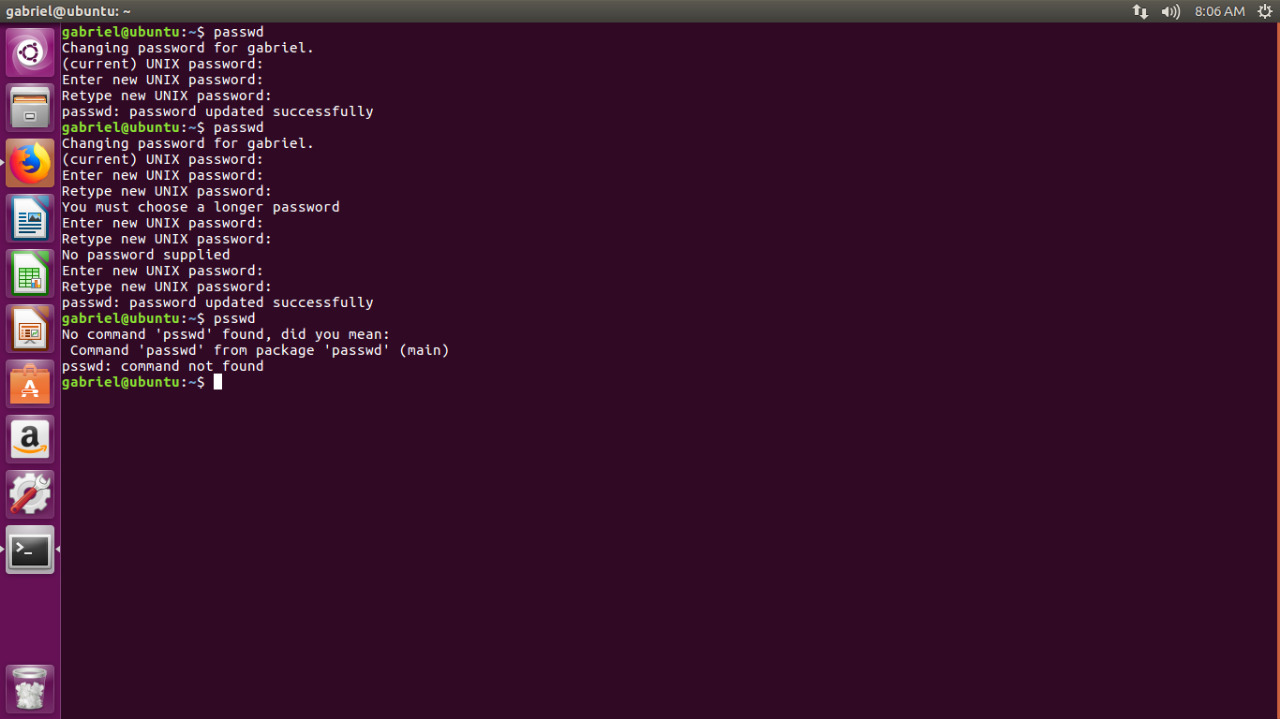
\includegraphics[trim= 0 295 666 0,clip,width=0.95\textwidth]{img/contrasena.jpg}
        \caption{contraseñas}
        \label{fig:my_label}
    \end{figure}
\section{Directorios}
    El comando (cd) es usado para acceder a un directorio específico, al usar cd blah, la terminal dice que no existe ningun directorio con este nombre. \\
    Al usar (cd..) sin espacio en medio también hace que la consola no pueda encontrar el comando.\\
    El comando PWD en linux devuelve la ruta en la que se está situado, se suele utilizar para saber en que parte de la estructura de directorios se encuentra el usuario.\\
    Al usar el comando (ls) se listan en pantalla todos los directorios en home, es decir el escritorio en Windows.\\
    Usando de manera adecuada el comando ( cd .. ) la terminal se devuelve al directorio anterior o accede al /home, listando el contenido de este directorio se encuentran folders como bin, boot, dev, y el más importante root.\\ 
    Al tratar de acceder al directorio root usando el comando (cd root) la terminal nos dice que es imposible ya que el usuario local no cuenta con los persimos de acceso al mismo. Jugando un poco con los directorios en /home parece ser que al único el cual el usuario local no tiene acceso es el de root.\\
    La forma mas fácil de acceder al root es con el comando (sudo -s).
    \begin{figure}[H]
        \centering
        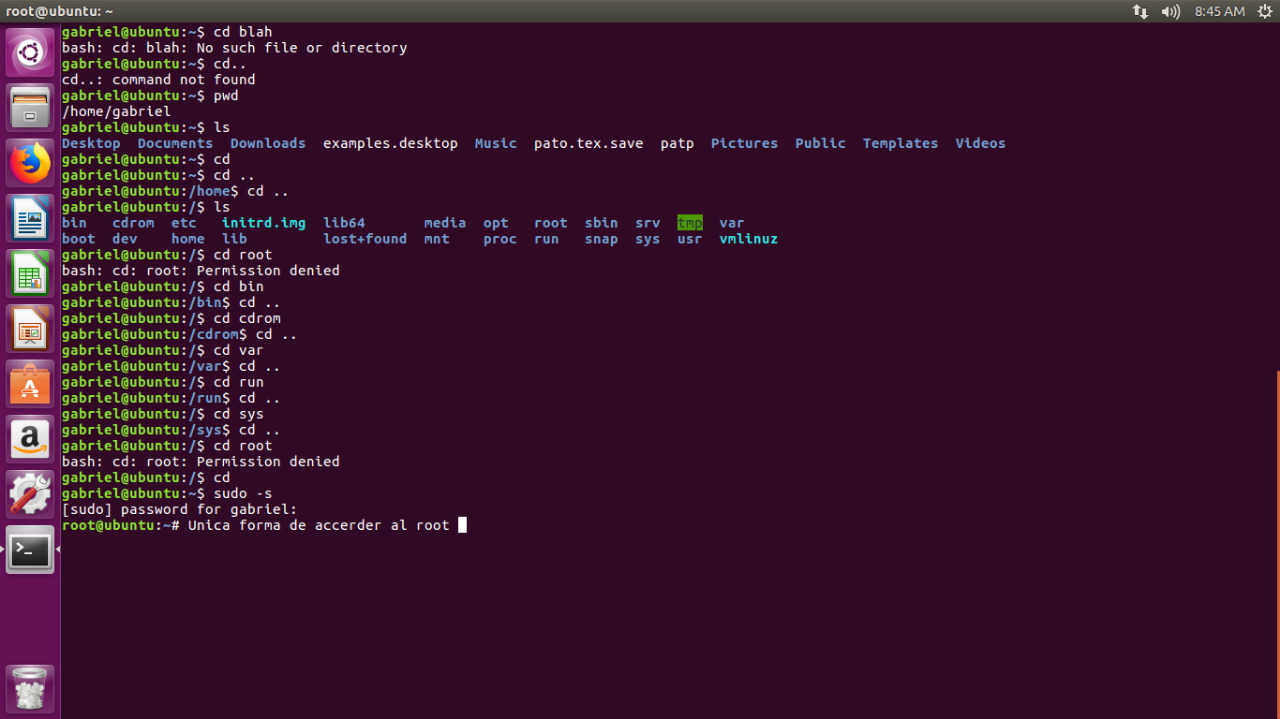
\includegraphics[trim= 0 175 230 0,clip,width=0.95\textwidth]{img/directorios.jpg}
        \caption{Jugando con los directorios}
        \label{fig:my_label}
    \end{figure}
\section{Archivos}
    Después de una exhaustiva busqueda por el /etc y dentro de la documentación de Linux, el archivo inittab es sumamente viejo y ha sido extraído de las distribuciones actuales de Linux, para acceder a esta información se usa man runlevel el cual contiene la misma información que el archivo inittab.
    \begin{figure}[H]
        \centering
        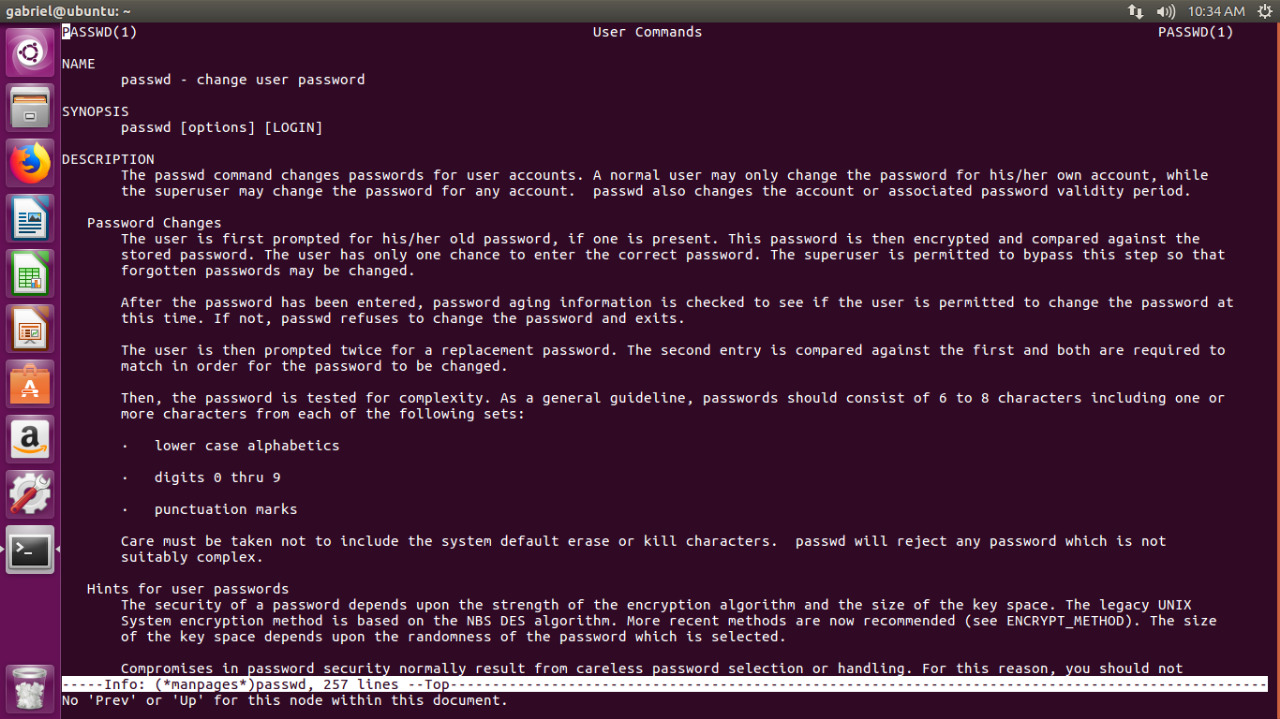
\includegraphics[trim= 0 175 0 0,clip,width=0.95\textwidth]{img/manpswd.jpg}
        \caption{Man psswd}
        \label{fig:my_label}
    \end{figure}
\section{Obteniendo Ayuda}
    El comando man en linux es usado para desplegar el manual de usuario para cualquier otro comando, es decir man ls, devuelve la documentación del comando ls el cual devuelve una lista de cosas dentro de un directorio.
    \begin{figure}[H]
        \centering
        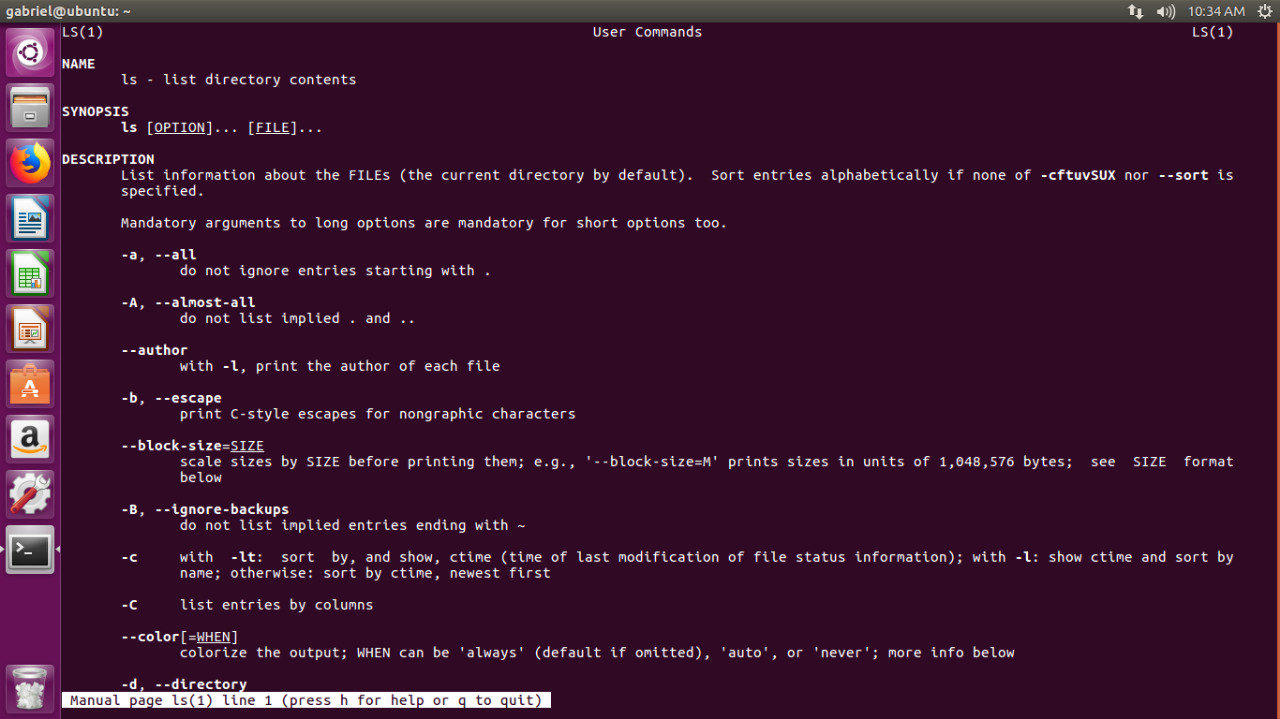
\includegraphics[trim= 0 175 0 0,clip,width=0.95\textwidth]{img/manRL.jpg}
        \caption{Man runlevel}
        \label{fig:my_label}
    \end{figure}
    
\section{Particiones}
\subsection{¿En qué partición está linux?}
    En el equipo de la Universidad se instaló en la partición número 7 /sda7
\subsection{¿Cuántas particiones hay en el equipo?}
    El computador de la Universidad cuenta con al menos 7 particiones diferentes. 
\subsection{¿Cuánl es el tamaño de su instalación de Linux?}
    El tamaño de la instalación de Linux es de 19Gb del cual están usadas solo 4.6Gb
    \begin{figure}[H]
        \centering
        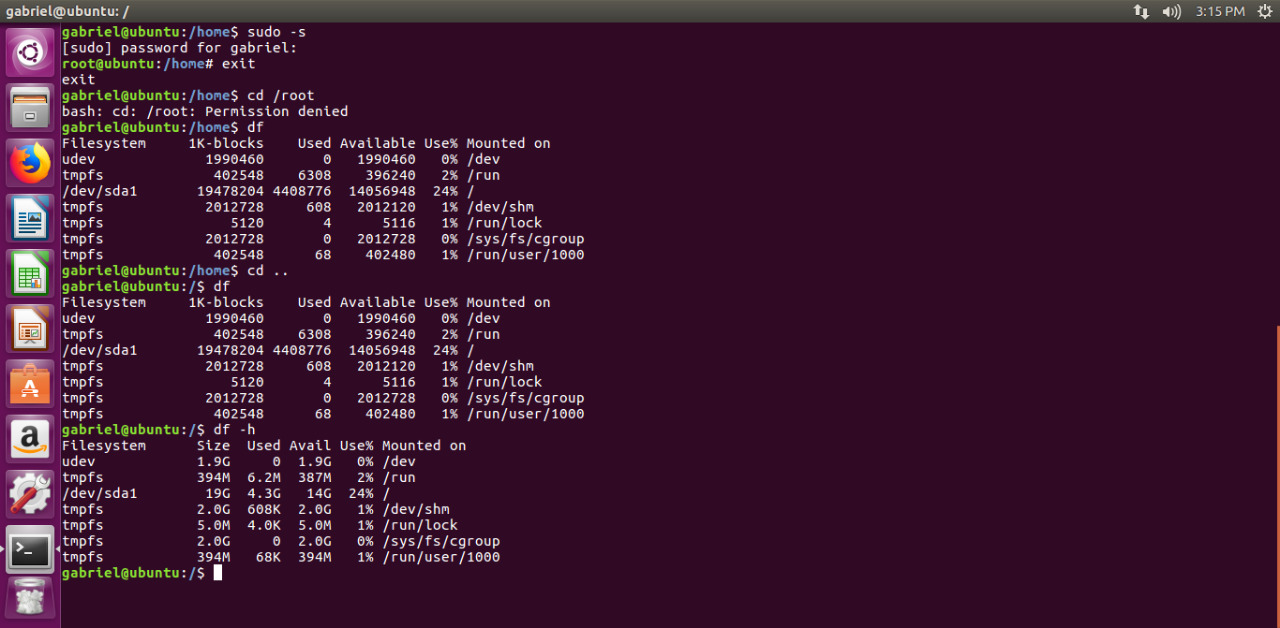
\includegraphics[trim= 0 40 750 420,clip,width=0.95\textwidth]{img/instalacion.jpg}
        \caption{Tamaño de instalación}
        \label{fig:my_label}
    \end{figure}
\section{Rutas}
    Se define como ruta absoluta aquella que contiene el punto exacto donde esta un archivo sin importar donde esté el usuario en un momento dado, mientras que la ruta relativa es "relativa" al folder donde esté el usuario en ese momendo dado. \\
    El "search path" son aquellas instrucciones que se pueden ejecutar sin necesidad de decirle a la terminal en qué lugar específico se encuentra este comando, es decir no es necesario indicar la ruta absoluta del comando para ejecutarlo.
    Si se exporta un (PATH=blah) entonces se estaría cambiando por completo el search path a blah por lo tanto al intentar listar el contenido no devolverá un error porque ls no esta en esta ruta.
    Para cambiar de usuario desde la terminal se usa el comando ( su - <nombre de usuario>), desde un usuario aparte para entrar al HOME de otro usando una ruta absoluta (cd /home/<nombre de usuario>/), y usando una ruta relativa estando en HOME entonces: (cd ../<nombre de usuario>).
    \begin{figure}[H]
        \centering
        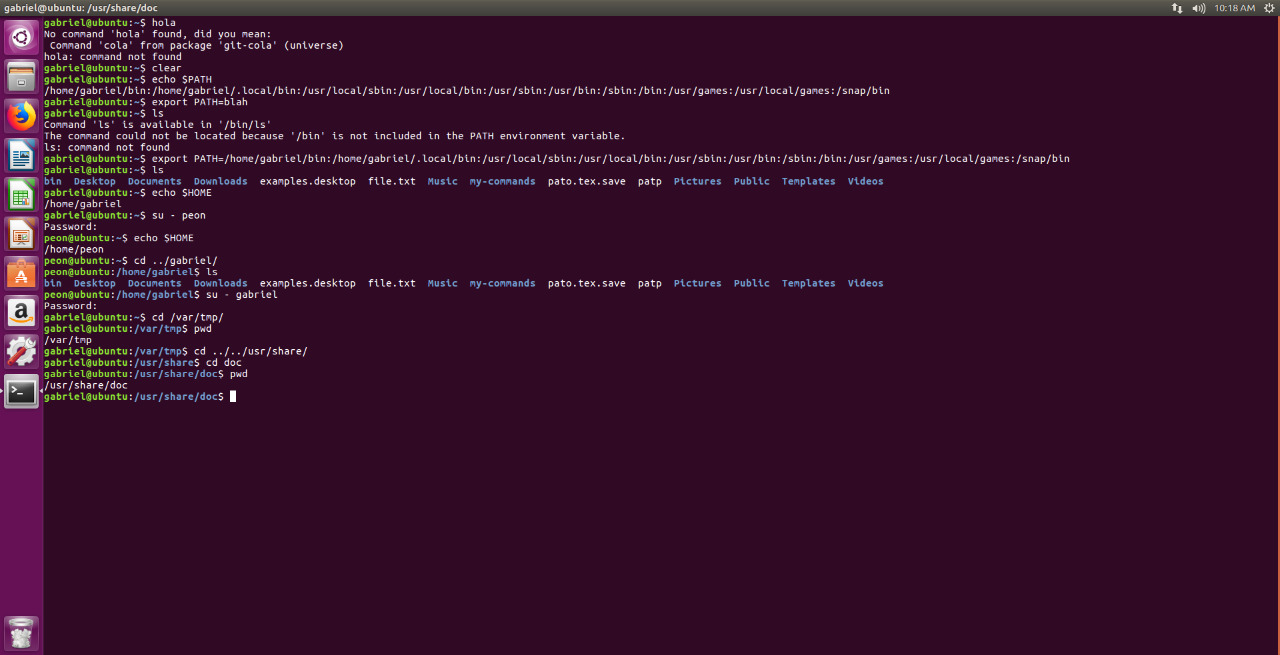
\includegraphics[trim= 0 240 650 0,clip,width=0.95\textwidth]{img/rutas.jpg}
        \caption{Trabajando rutas absolutas y relativas}
        \label{fig:my_label}
    \end{figure}
\section{Tour del sistema}
    \subsection{Pasando al /proc y encontrando CPU y RAM}
        Se usa el comando cd /proc para entrar al directorio y aqui se usa el cat para abrir los documentos meminfo y cpuinfo.
        \begin{figure}[H]
            \centering
            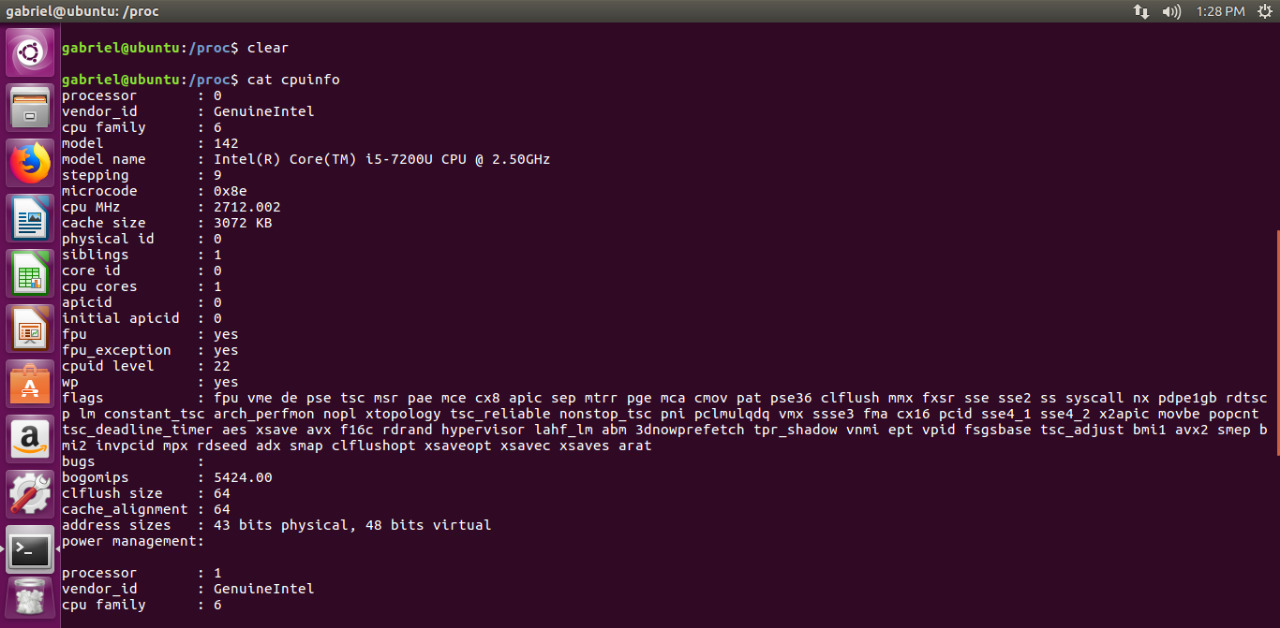
\includegraphics[trim= 0 240 650 0,clip,width=0.95\textwidth]{cpu.jpg}
            \caption{CPU (Intel core i5)}
            \label{fig:my_label}
        \end{figure}
        Aqui también se puede obtener la Swap Memory la cual es una extensión de la memoria real de la computadora. Esto permite que el equipo pretenda tener más memoria de lo que en realidad tiene.
        \begin{figure}[H]
            \centering
            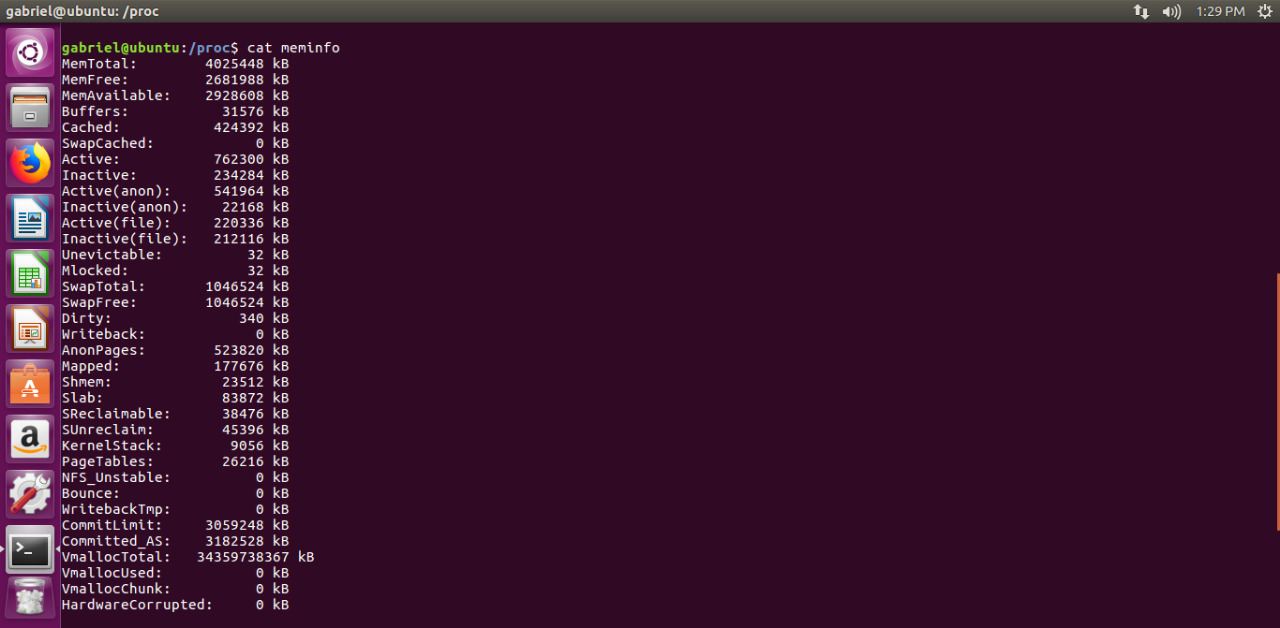
\includegraphics[trim= 0 320 750 0,clip,width=0.95\textwidth]{img/ram.jpg}
            \caption{Memoria Ram}
            \label{fig:my_label}
        \end{figure}
    \newpage
    \subsection{Drivers}
        En Linux los "drivers" se conocen con el nombre de modulos. Un controlador o modulo, es un programa informático que permite al sistema operativo interaccionar con un periférico, haciendo una abstracción del hardware y proporcionando una interfaz para utilizar el dispositivo.
        \begin{figure}[H]
            \centering
            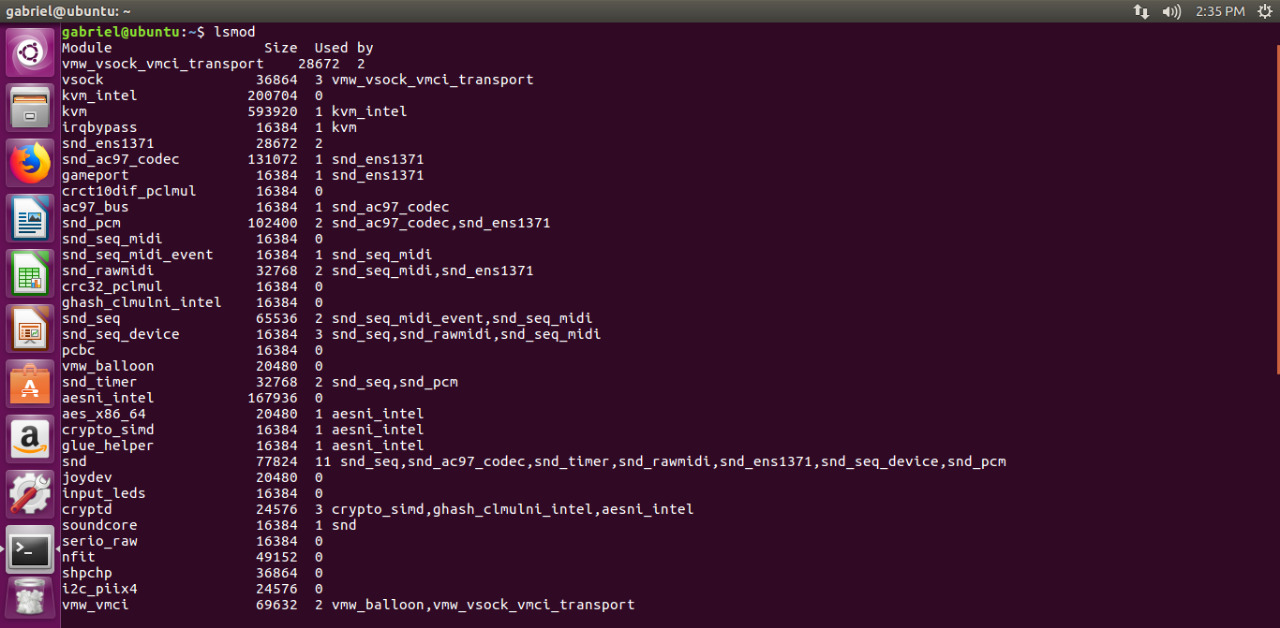
\includegraphics[trim= 0 320 750 0,clip,width=0.95\textwidth]{img/drivers.jpg}
            \caption{Drivers}
            \label{fig:my_label}
        \end{figure}
    \subsection{Hora y FileSystem}
        Cuanto tiempo ha estado encendido el sistema, para esto se usa el comando (last reboot). El filesystem es el sistema de archivos que maneja el equipo.
        \begin{figure}[H]
            \centering
            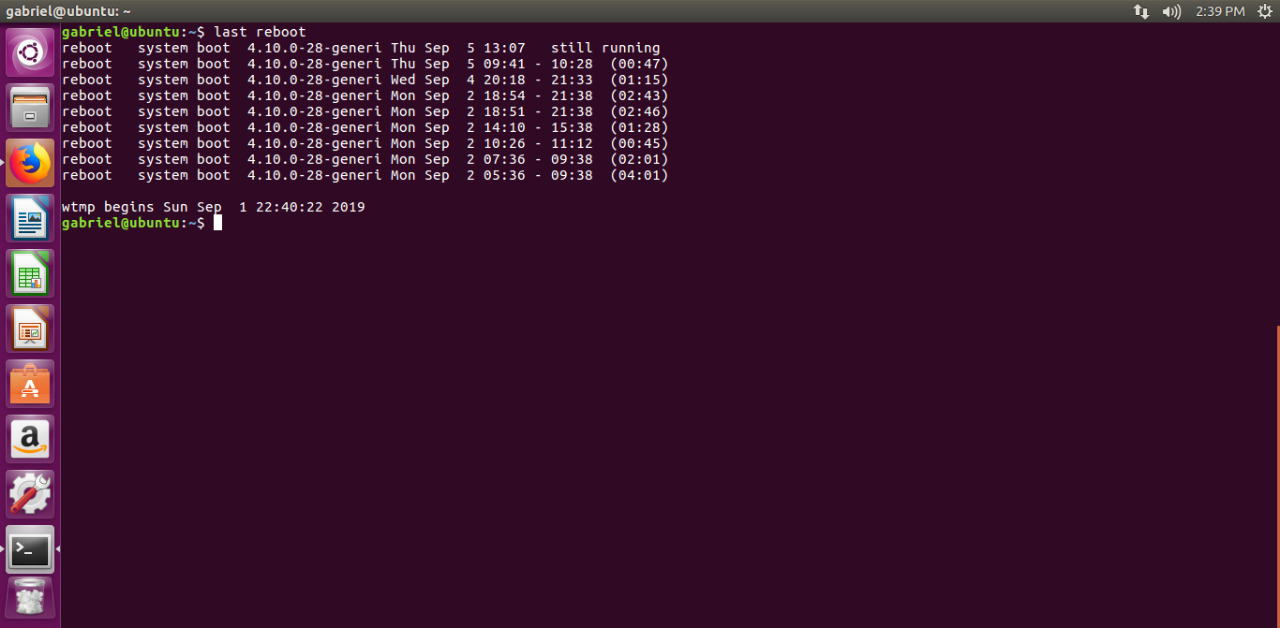
\includegraphics[trim= 0 390 580 0,clip,width=0.95\textwidth]{img/hola.jpg}
            \caption{Hora del sistema}
            \label{fig:my_label}
        \end{figure}
        Para el sistema de archivos se usa el comando ( df -hT ). En la segunda columna de la salida se puede observar el tipo de archivos el cual contiene el equipo.
        \begin{figure}[H]
            \centering
            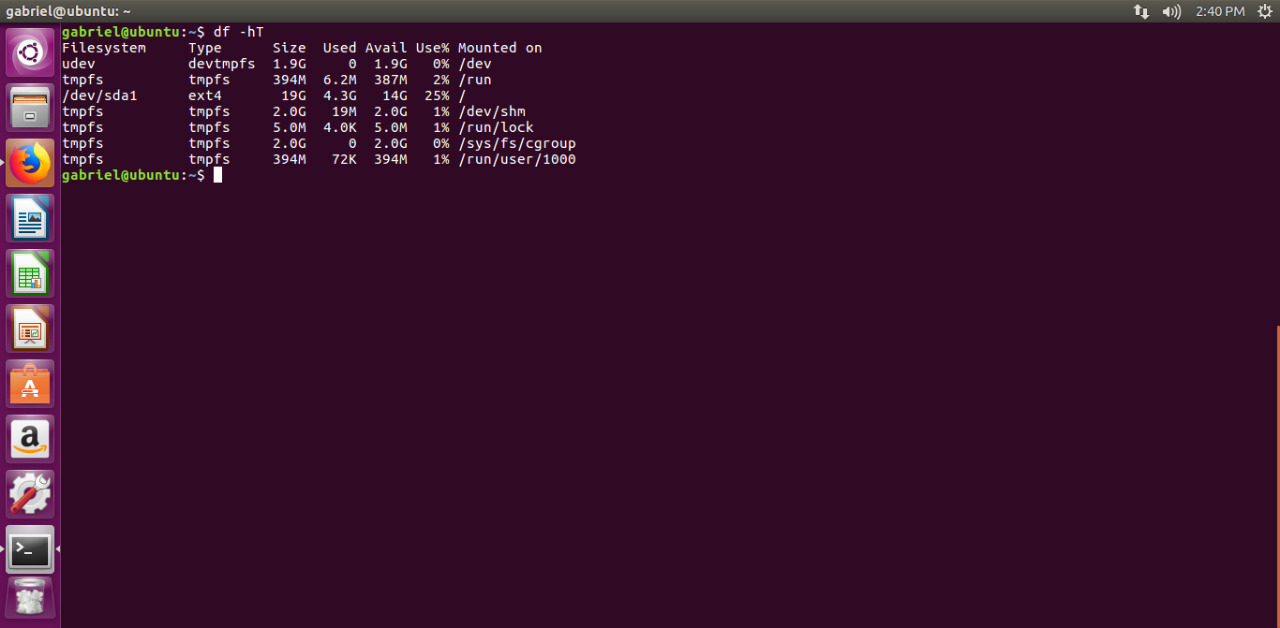
\includegraphics[trim= 0 430 580 0,clip,width=0.95\textwidth]{img/files.jpg}
            \caption{Sistema de Archivos}
            \label{fig:my_label}
        \end{figure}
        \newpage
        \subsection{Nivel de ejecución}
            El sistema usado para este laboratorio es UBUNTU en el cual solo existe el archivo /etc/init.d , así va a ser en todas las plataformas de debian. El nivel de ejecución por defecto es el 5 el cual tiene multiuser mode/networking pero además tiene un GUI para que el usuario trabaje con mayor facilidad. El tiempo que se guardan los archivos sobre la actividad del usuario es de 12 semanas, despues de esto el sistema operativo los empaqueta y los guarda y se repite el proceso. La versión de lanzamientos del Linux usado es 16.04 para ver la misma se usa el comando lsb\_release -a
            \begin{figure}[H]
            \centering
            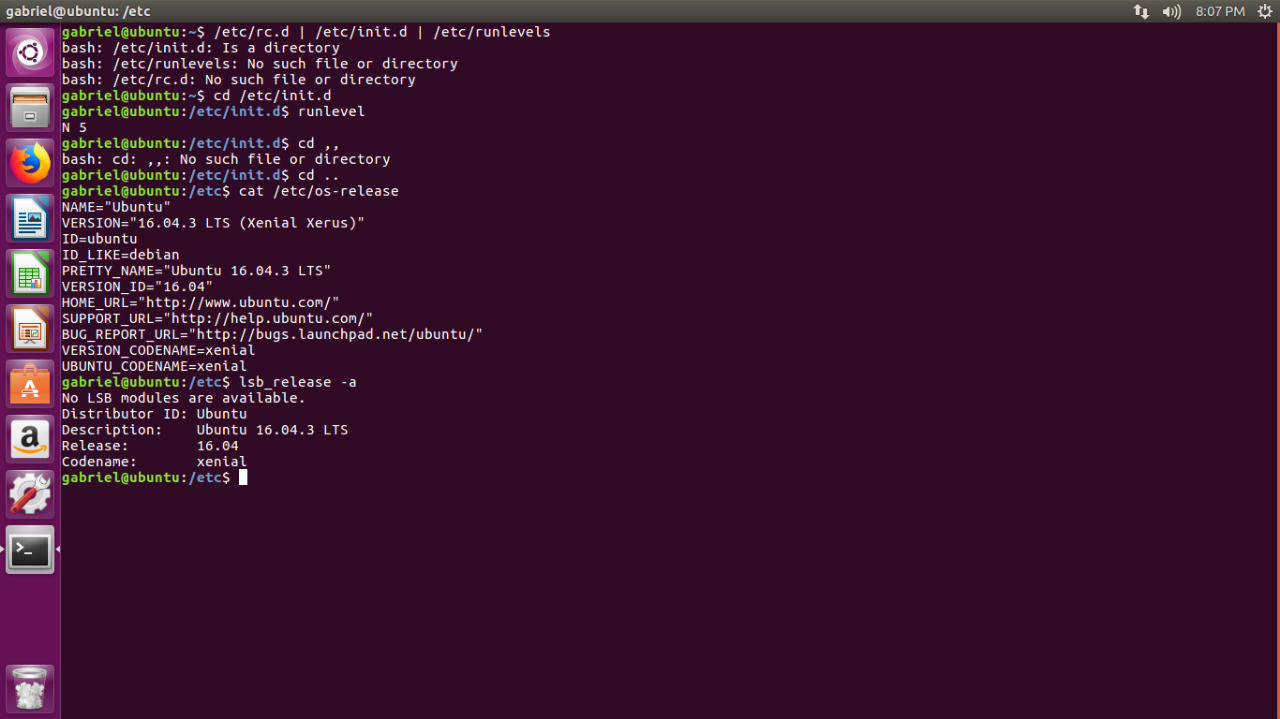
\includegraphics[trim= 0 220 580 0,clip,width=0.95\textwidth]{img/tour.jpg}
            \caption{Tour del sistema}
            \label{fig:my_label}
            \end{figure}
            Para hallar si existen mensajes del dia en el directorio motd se usa /etc/update-motd.d y una vez estando en esta ruta, se usa el comando sudo ./50-landscape-sysinfo para obtener acceso al mensaje dentro de la carpeta. 
            Para la cantidad de usuarios se usa el comando compgen - u y adicionalmente el wc -l para que devuelva el numero total, es impresionante ver que son 42 usuarios diferentes, algunos: root, daemon, bin, sys, entre otros.Para el numero de grupos al igual que para los usuarios se usa el comando grops concatenado por un | y wc -w.
            Para la zona horario se hizo uso del comando whereis <localtime> para hallar la ruta.
            \begin{figure}[H]
                \centering
                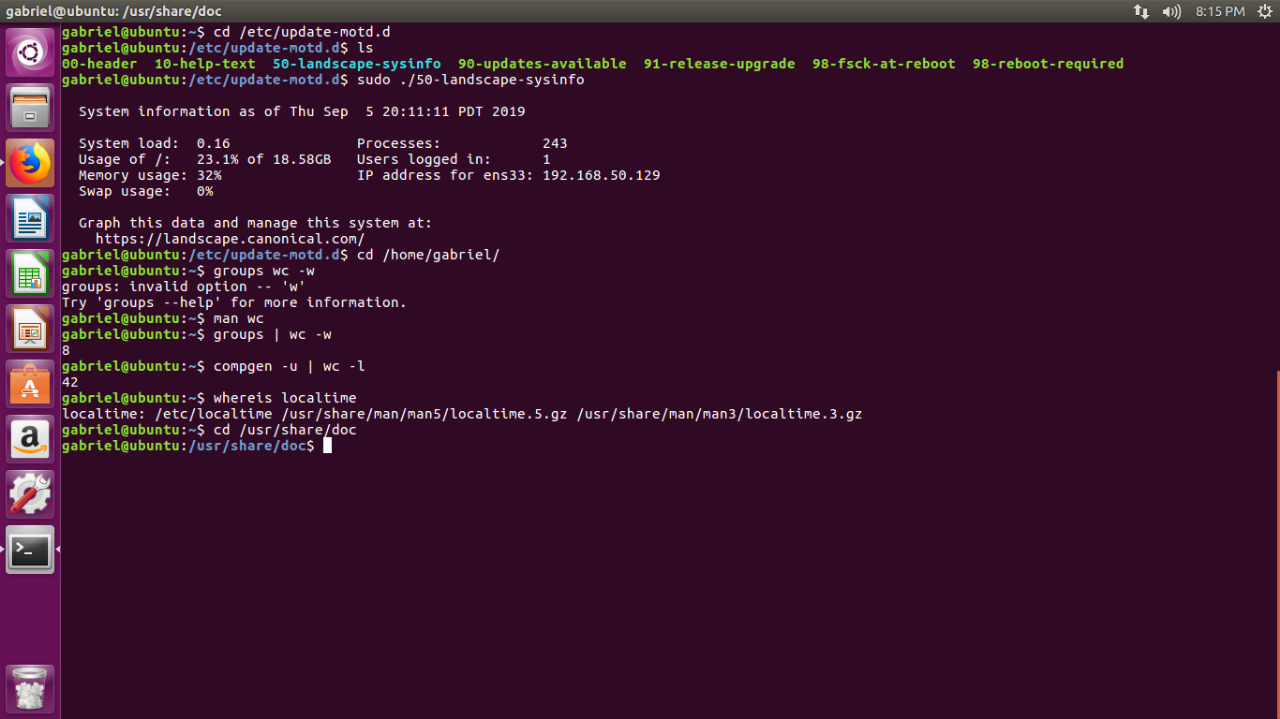
\includegraphics[trim= 0 250 400 0,clip,width=0.95\textwidth]{img/men.jpg}
                \caption{Numero de usuarios, mensajes del dia y zona horaria}
                \label{fig:my_label}
            \end{figure}
        \subsection{GNU coreutils}
            Coreutils trae muchas reimplementaciones para las herramientas básicas como ls, cat y rm.
        \subsection{Versión de BASH}
            La salida que da el equipo al utilizar el comando echo \$ BASH\_VERSION (4.3.48(1)-release)
\section{Manipulación de Archivos}
    Para crear un directorio nuevo se usa el comando mkdir <nombre>. Se puede poner al nivel de /home unicamente si se trabaja desde root es decir usando el superusuario. Para copiar todos los archivos de /usr/share/pixmaps/ en la carpeta nueva se debe usar el comando cp -r el -r es para que lo haga de manera recursiva ya que se quiere copiar directorios. Para listar el contenido en orden algabético en reversa se usa el tradicional ls -r, -r en este caso cumple con esa función. El archivo XPM es uno de archivos de la categoría Archivos de imagen de mapa de bits. Su nombre completo es X11 Pixmap Graphic.
        \begin{figure}[H]
            \centering
            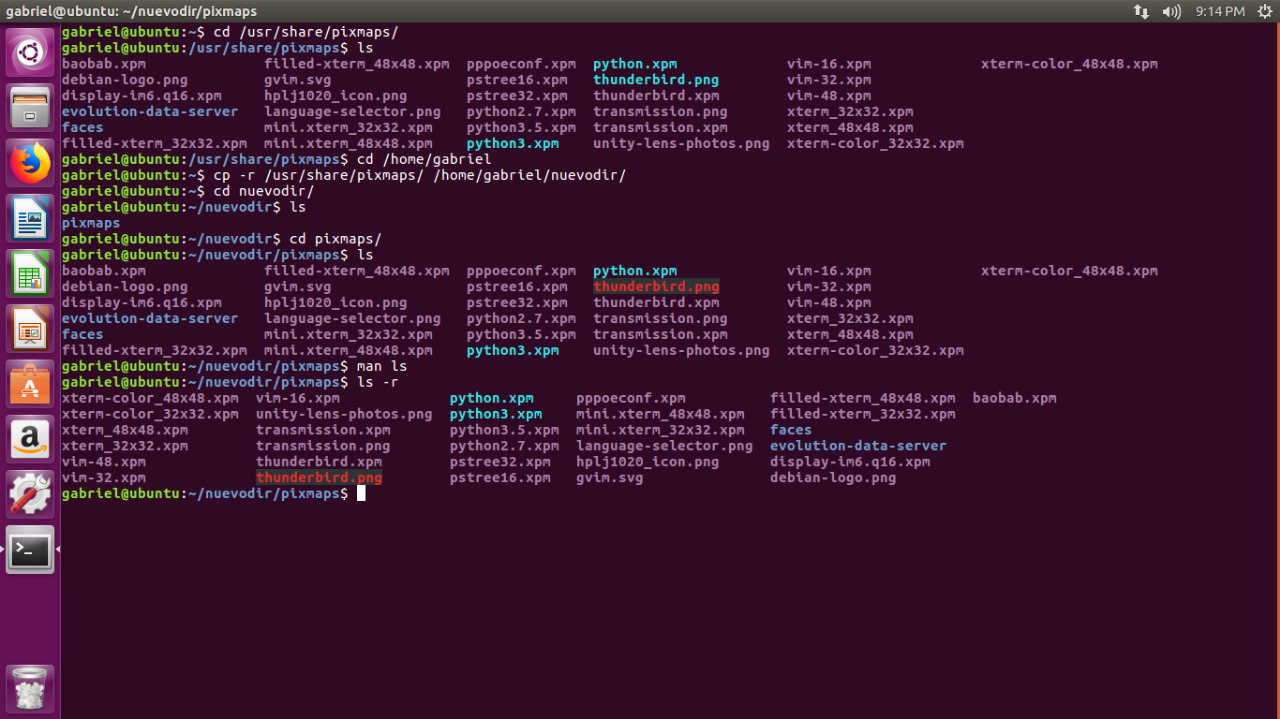
\includegraphics[trim= 0 200 250 0,clip,width=0.95\textwidth]{img/cp.jpg}
            \caption{Copiando pixmaps}
            \label{fig:my_label}
        \end{figure}
    Se creó un directorio nuevo en /home y se procedió a hacer la copia de /etc usando sudo para que no existan errores, una vez la copia hecha para buscar y guardar todos los documentos que empiecen con letra mayúscula o bien minúscula se usa un codigo, one liner para facilitar el trabajo: find ./ -name '[a-z]*' -exec mv -t ../lower/ {} +, en el caso de las minúsculas y find ./ -name '[a-z]*' -exec mv -t ../upper/ {} + para las mayúsculas.
        \begin{figure}[H]
                \centering
                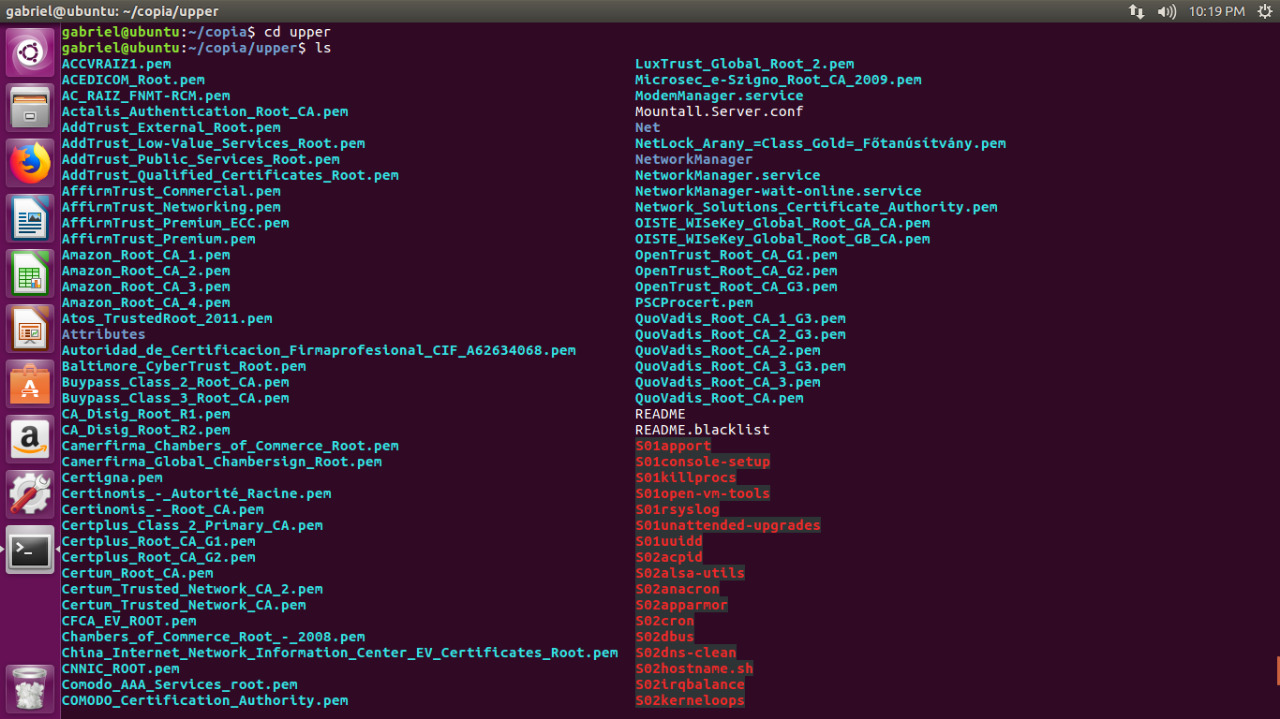
\includegraphics[trim= 0 550 350 0,clip,width=0.95\textwidth]{img/upper.jpg}
                \caption{Mayúsculas}
                \label{fig:my_label}
        \end{figure}
        \begin{figure}[H]
            \centering
            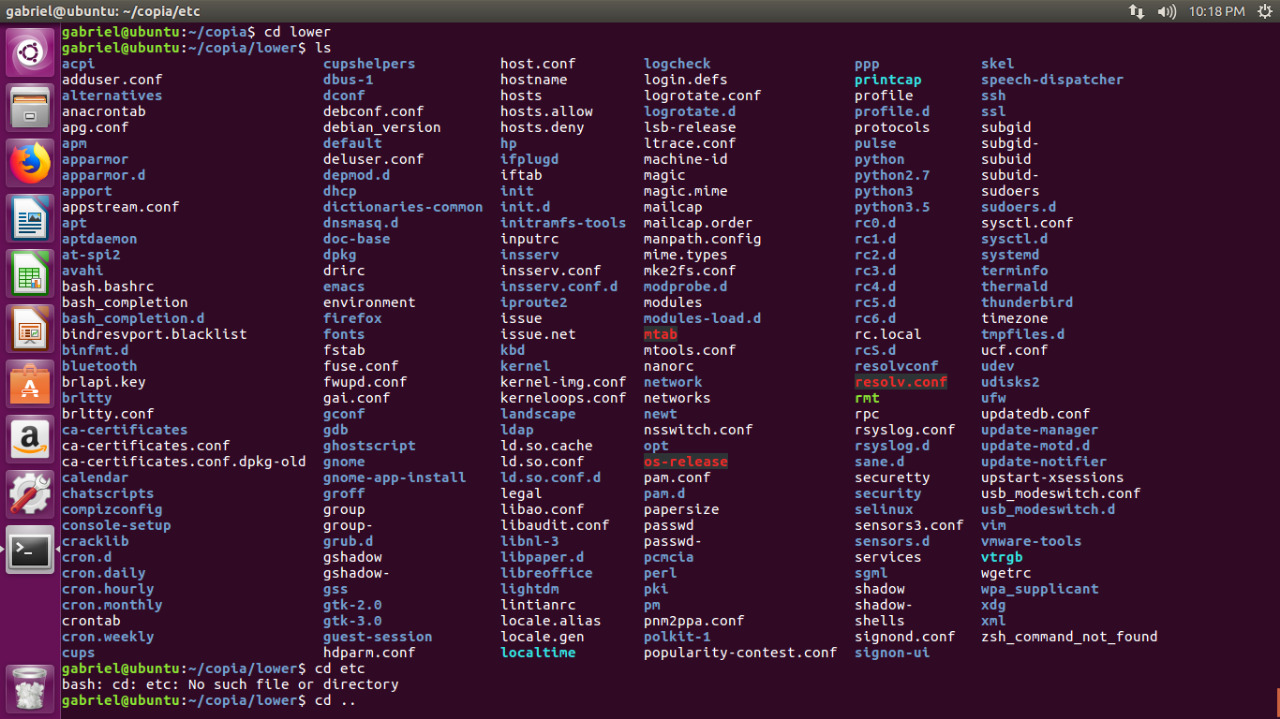
\includegraphics[trim= 0 550 350 0,clip,width=0.95\textwidth]{img/lower.jpg}
            \caption{Minúsculas}
            \label{fig:my_label}
        \end{figure}
    Se procede a borrar el directorio que se creó para este ejercicio, para esto se usa el comando rm -r para hacerlo de forma recursiva.
        \begin{figure}[H]
            \centering
            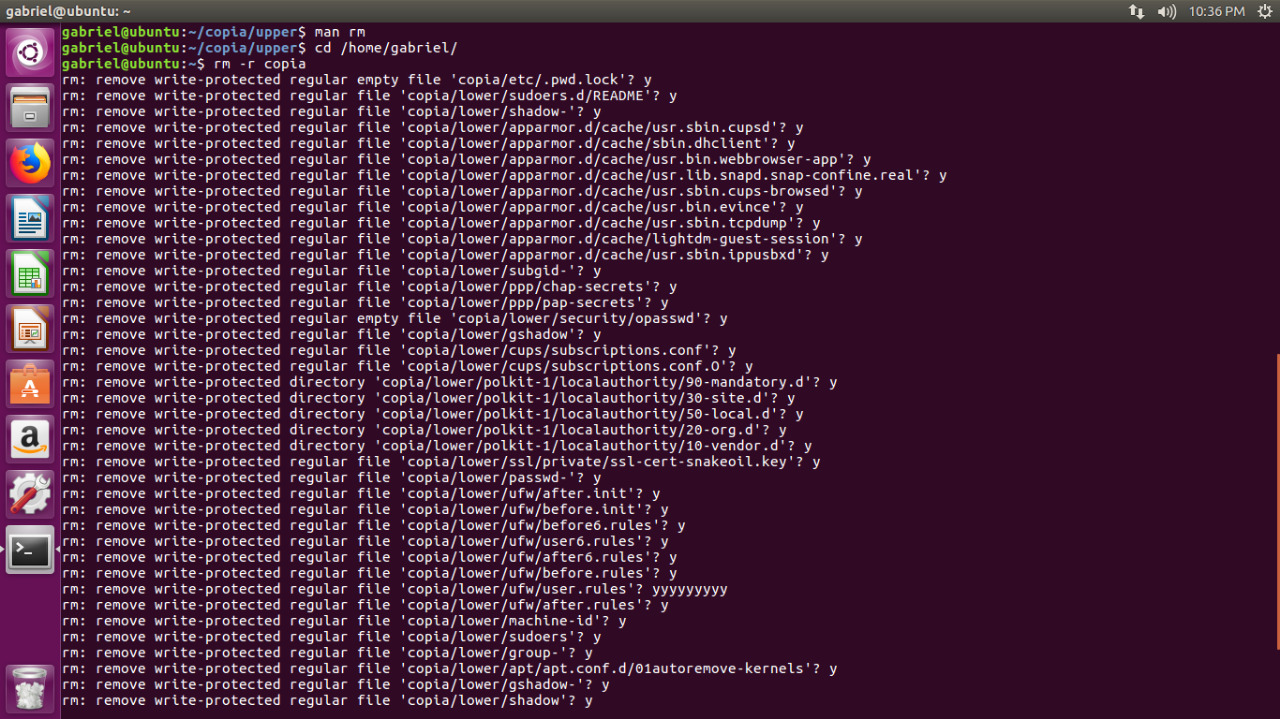
\includegraphics[trim= 0 520 300 0,clip,width=0.95\textwidth]{img/borrando.jpg}
            \caption{Borrando el directorio}
            \label{fig:my_label}
        \end{figure}
        Se usa el comando cat /etc/init.d/* | grep -i "font server", pero devuelve nada, por lo tanto esto quiere decir que no existe la palabra font server no existe en /init.d.\\
        El archivo /etc/sendmail.cw define nombres alternativos de host. Define procmail como el programa de correo local en el servidor.
        Usando los comandos mv /home/<myuser>/varcache /home/var/cache, rm -f /var/cache,ln -s /home/var/cache /var/cache, se logra hacer el enlace simbolico del sistema.
        
    
\section{Permisos}
    \subsection{¿Se pueden cambiar los permisos en /home?}
        Sí, se usa el comando chmod 777 para abilitar los permisos que se requieran al directorio seleccionado. 
    \subsection{¿Cuál es el modo estándar de creación de archivos?}
        Cuando un usuario crea un archivo o directorio en Linux, el sistema lo crea con un set standár de permisos,en este caso el que usa Linux y UBUNTU es UMASK y es usado para controlar los persos los cuales tendrán los archivos creados. 
        Para cambiar los permisos de /etc como en el punto anterior se usa el comando chmod 777 /etc para darle todos los permisos disponibles.\\
        Para cambiar los permisos de /.bashrc se debe usar el comando sudo chmodd 440 para unicamente habilitar los permisos de lectura del directorio para el usuario y el grupo.\\
        El comando locate root no se puede usar sin usar sudo, y devuelve la ruta absluta del directorio madre root.
        No es posible hace in enlace simbolico con root ya que el usuario no tiene permiso para el mismo.
        
        
        
        
    
    

    
\end{document}
